\clearpage
\thispagestyle{empty}
\addcontentsline{toc}{chapter}{\hspace{6mm}\textbf{CHAPTER 3 \hspace{8mm} METHODOLOGY \hspace{7.3cm}}}

\begin{center}
	\textbf{{CHAPTER 3}}\\
	\vspace{-1ex}
	\textbf{METHODOLOGY}
	\vspace{-3ex}
\end{center}
\subsection{Research Methodology}
\vspace{-2ex}
The software development methodology to be utilized in the study is Extreme Programming (XP). It is a software development methodology that provides values and principles to guide the team behavior and improves the quality of the results of the study.

The researchers used this methodology because it is a pragmatic approach to program development that emphasizes results first and takes an incremental, get-something-started approach to building the product, using continual testing and revision.

\begin{figure}[H]
	\centering
	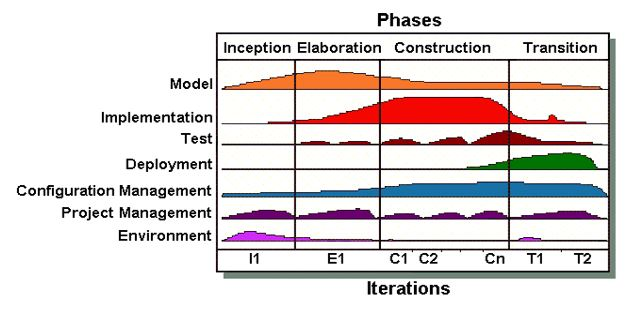
\includegraphics[width=15cm,height=9cm]{image/3-1.jpg}
	\caption{Rational Unified Process}
\end{figure}

\noindent\textbf{Phase 1:  Inception Phase}\\
\hspace*{1.5cm}The Inception phase is where the researchers get familiarity with the project goal and scope. It helps determine the project feasibility, what customer wants, and how the researchers will get into more resource consumable phase.
	
The researchers planned to integrate GetOldTweets in the system for the collection of data. To make sense of the collected data, topic modelling should be done. For the topic modelling, the researchers integrated Mallet. To analyze the data, visualization is needed. To visualize the generated topic models, the researchers planned to use GraphStream.
	

\noindent\textbf{Phase 2: Elaboration Phase}\\
\hspace*{1.5cm}This phase is one of the crucial parts in the development of the study since collecting the most significant requirements for the system takes place. In this phase, the researchers should be able to define and baseline the architecture of the system in order to provide a stable basis for the bulk of the design and implementation effort in the Construction Phase. 

This is where the researchers determine the requirements of the proposed system. This can be presented by the various modules/features based on your presented objectives.

\begin{figure}[H]
	\centering
	\caption{Flowchart}
	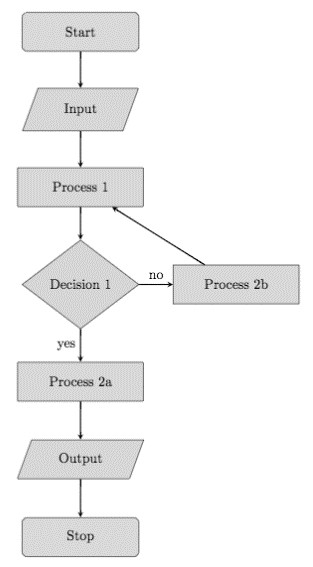
\includegraphics[width=7cm,height=11cm]{image/cs_flowchart.jpg}
\end{figure}


\noindent\textbf{Phase 3: Construction Phase}\\
\hspace*{1.5cm}The Construction Phase is about cost-efficient development of a complete product and operational version of the system that can be deployed in the user community. It is where the researchers develop a complete product that is ready for transition to its community. 
	
The researchers translated both the initial logical and physical designs to actual system development. The Java programming language was used by the researchers in the development of the system and tools were utilized to accomplish goals. The researchers used tools to accomplish our goals. For the data gathering, we used GetOldTweets1 an unofficial Java library for the Twitter 20 API and we used MAchine Learning for LanguagE Toolkit or MALLET2 for the topic modelling. MALLET is a Java-based package for statistical natural language processing, document classification, clustering, topic modelling, information extraction, and other machine learning applications to text. For the visualization, the researchers used GraphStream3, it is a tool for generating graphs, links and networks. We also used jFreeCharts for the visualization of the frequency of the words.

\subsection{Design of Software}
\vspace{-2ex}Software design is the process of transforming user requirements into appropriate abstracts which helps the researchers in designing, coding and implementing the developed software.

\begin{figure}[H]
	\centering
	\caption{Conceptual Framework}
	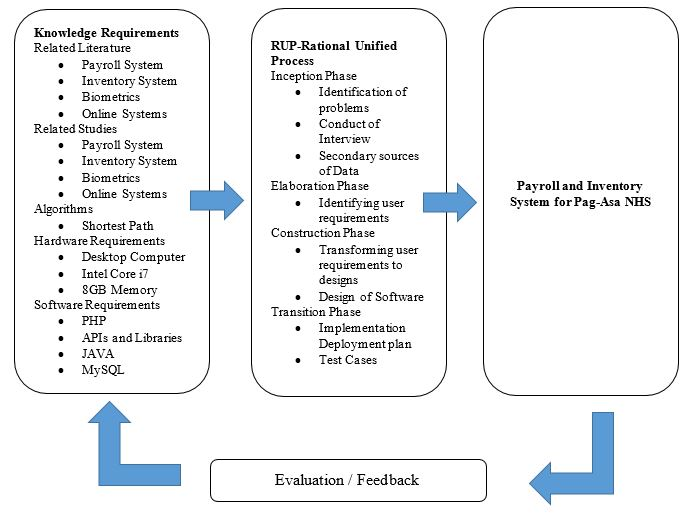
\includegraphics[width=15cm,height=11cm]{image/3-3.jpg}
\end{figure}
\noindent\textbf{Phase 4: Transition Phase}\\
\hspace*{1.5cm}The purpose of the transition phase is to transition the software product to the user community. In this phase the researchers validate the new system against user expectations. 
	
The researchers prepared test cases to ensure that the developed system requirements were met…

\begin{table}[H]
	\centering
	\caption{Software Requirements}
	\begin{tabular}{ | C{4cm} | C{6cm} | C{4cm} |} 
		\hline
		Component & Minimum	& Suggested \\
		\hline
		Browser & Google Chrome & Google Chrome \\
		\hline
		Apache, MySQL  and PHP	& Version 5 & Version 5.5 or latest \\
		\hline
		
	\end{tabular}
\end{table}

\begin{table}[H]
	\centering
	\caption{Hardware Requirements}
	\begin{tabular}{ | C{4cm} | C{6cm} | C{4cm} |} 
		\hline
		Component & Minimum	& Suggested \\
		\hline
		Disk Space & 10GB & 30GB \\
		\hline
		Memory Requirement & At least 512 MB of Random Access Memory (RAM) & 1GB of RAM \\
		\hline
		Processor &	Intel or AMD Processor, at least 1.06 GHz	& Intel or AMD Processor, 1.7 GHz \\
		\hline
	\end{tabular}
\end{table}

Every computer system has requirements in terms of Software and Hardware used for better implementation. In this case, the researchers listed in the table above the required software and hardware to be used in the proposed system.

%For your NLP process, you may include under the implementation phase of your methodology the following but not limited to: Data Collection, Data Filtering, Data Processing, Data Analysis. These NLP processes may also integrate discussion of the algorithm used, notations and formulas, evaluation methods, tools used, and other NLP concepts.